\chapter{Methodology}\label{Methodology}
\section{motor learning model}
This work optimizes a motor spicing model introduced by Spüler et al. \cite{sebastianPaper}\cite{sebastianPaper} which is an extension of the work of Chadderdon et al. \cite{chadderdonNeuronalModel}. The model presents a biologically realistic model of the motor cortex, which uses reinforcement learning to reach a target angel with a simulated forearm.
As a standard reinforcement model \cite{reinforcementlearning}\cite{chadderdonNeuronalModel} it consists of an actor, that maps perceptions to actions a environment that reacts and a critic providing reward or punishment feedback to the actor. Spüler et al. and Chadderton et al. realized the environment as a forearm model with a one degree of freedom joint. Therefore the forearm could be moved either up or down. The joint angle limited by 0\degree and 135\degree. Whereby 0\degree means fully straightened and 135\degree means fully flexed. The actor got implemented with a spiking neural network. A spiking neural network is a weighted connected graph with some input and output nodes. Each edge is called a connection and each vertex called a neuron. The network calculates a time depending mapping from some input to output values.
Figure \ref{fig:reinforcementcircle} gives an overview over all components of the model as also of the reinforcement learning process.
 %TODO cite! oder ausführlicher erklären. ANN and SNN. Oder al bekannt annehmen...
%vielleicht hier erst grobe struktur erklären, dann neurons im detail.
Each neuron in this model represents an either excitatory or inhibitory dynamic unit. Excitatory neurons excite connected neurons, while inhibitory neurons inhibit connected neurons.
The dynamics or in other words the time depending state of each neuron is represented by the membrane potential $V_m(t)$.$V_m(t)$ is modelled by an differential equation introduced by Izhikevich \cite{izhikevichSimpleModel}, which is a good and efficient approximation of the Hodgkin-Huxley model \cite{hodgkinHuxleyModel}. Izhikevich's model slightly adapted by Spüler et al. with noise is described as follows (variable names changed):
\begin{align*}
	V_m(t)' &= 0.04 V_m(t)^2+5V_m(t)+140-u+I(t)+V_n(t)\\
	u(t)' &= a(b\cdot V_m(t)-u(t))\\
	&\text{reset after spike:}\\
	\text{if } v&\geq V_t,\text{ then}
	\begin{cases}
	1 & \leftarrow V_r\\
	0 & \leftarrow u+d\\
	\end{cases} 
\end{align*}
where $u$ represents the membrane recovery variable. $I$ defines the synaptic input currents. That is the sum of weighted inputs to a neuron.(TODO ref to ANN fundamentals) The firing pattern of a neuron depend on the choice of parameters $a,b,d,V_r$ and $V_t$. Different resulting spiking patterns can be seen in figure \ref{fig:spikingpatterns}. $V_r$ is the resting potential of the neuron. $V_t$ the spiking threshold. $V_n$ is a 300Hz noise input that leads to motor babbling. That is, network send output signals although no input signal is given. This behaviour is important for reinforcement learning since if the actor doesn't produce any actions the critic isn't able to give feedback \cite{chadderdonNeuronalModel}.The parameter a,b,c,d are chosen as one can shown in table \ref{table:DynamiModelParams}.
%allgemein fehlt oft der Bezug auf den Motor cortex und ob das dort ähnlich  ist
%TODO should be past tense because was done and not universal valid 
\begin{table}[h]
	\centering
	\begin{tabular}{ |c||c|c|  }		
		\hline
		Parameter & Excitatory & Inhibitory \\
 		\hline
 		$a$&$0.02$& $0.02+0.08r_i$\\
 		$b$&$0.2$& $0.25-0.05r_i$\\
 		$d$&$8-6\cdot r_i^2$& $2$\\
 		$V_r$&$-65$& $-63$\\
 		\hline
	\end{tabular}
	\caption[Dynamic model's parameters ]{Parameters used in the dynamic model }
	\label{table:DynamiModelParams}
\end{table}

%Noice:
% how noice is calculated not important

$r_i$ is uniform distributed in  $[0,1]$. For excitatory neurons moving $r_i$ from $0$ to $1$ leads to a transition from a regular to a chattering spiking pattern. For inhibitory neurons from a fast to a low-threshold spiking pattern. Examples of those patterns can be seen in (TODO ref appendix.).
The neurons are further divided into 5 logical groups: proprioceptive (P), excitatory sensory (ES), inhibitory sensory(IS), excitatory motory (EM) and excitatory sensory (IS) neurons.  Spüler's et al. model contains 48 P, 96 ES, 32 IS, 48 EM and 32 IM cells. Which leads to a total amount of 256 neurons.
Each logical group is connected with a specific probability as shown in \ref{table:SpuelerConnectionProbs}:

\begin{table}[h]
	\centering
		\begin{tabular}{ |c|c|c|c|c|c|  }
			\hline
			   & P &  EM  & IM   & ES   & IS    \\ \hline
			P  & 0 &  0   & 0    & 0,1  & 0      \\
			EM & 0 &  0   & 0,43 & 0    & 0     \\
			IM & 0 & 0,44 & 0,62 & 0    & 0      \\
			ES & 0 & 0,08 & 0    & 0    & 0,43   \\
			IS & 0 &  0   & 0    & 0,44 &  0,62 \\ \hline
		\end{tabular}
	\caption[Spüler's et al. model's connection probabilities ]{Connection probabilities of neuron types in the model of Spüler's et al.}
	\label{table:SpuelerConnectionProbs}
\end{table}
%firing rates:
% not important
%
Based on these connections the resulting network is shown in figure \ref{fig:modelstructur}.


% TODO structure: RF learning, Arm, neuro model. Dynamics, movement coding, learning

The motor control cycle works as follows: A new movement angle is encoded by EM neurons, after a time gap of 50 ms the forearm moves. At the same time reward or punishment is send. After a second time step of 25 ms the new position angle is encoded by the proprioceptive cells. \cite{sebastianPaper} grounds the time gaps on peripheral and sub cortical processing delays. Why there is an additional delay for the P cells to fire but not for the reward keeps ungrounded. The whole system works with a frequents of 0.02kHz. That means the EM neurons encode a new angle every 50ms. An overview of this process can be seen in figure \ref{fig:timing}.
The time needed by EM cells to encode a new angle is again 50ms. EM cells are parted into two equal sized groups of 24 neurons. The first 24 are in the first group the next 24 in the second. Each firing of a cell in the first group leads to an 1\degree  downward motion of the arm; in the lower part it leads to an 1\degree  upward motion. Over the time window of 50ms all spikes in each group are summed up. The resulting movement angle the difference of those sums.
Whether reward or punishment is send by the critic is decided whether the distance $\Delta\theta_t $of the current angle $\theta_t$  to the target angle $\theta_{target}$ got smaller or higher compared to the mean of the last two differences $\Delta\theta_{prev}$. This can be seen in the following formula:
\begin{align*}
	\Delta\theta_t &= |\theta_t-\theta_{target}|\\
	\Delta\theta_{prev} &= \left| \dfrac{\theta_{t-1}+\theta_{t-2}}{2} -\theta_{target}  \right |\\
	\text{critic response} &= 
	\begin{cases}
	\text{reward} &  \quad \text{if } \Delta\theta_t < \Delta\theta_{prev}\\
	\text{punishment}& \quad \text{if } \Delta\theta_t > \Delta\theta_{prev}\\
	\text{no response}& \quad \text{if } \Delta\theta_t = \Delta\theta_{prev}\\
	\end{cases}
\end{align*}
Note that reward or punishment doesn't influence every connection. Connections according to the Hebbian theory \cite{originalHebbianLaw} are only able to learn if a post-synaptic spike followed a pre-synaptic spike in the 50 ms where the movement to the current angle got encoded. Further on only connections from ES to EM neurons are able to learn. (TODO Why find prove ).  Reward or punishment increases or decreases a weight scale factor of each connection that is able to learn. For more informations look Appendix. TODO just copy picture.
A weight lies in the interval [0,5].\\
Depending on the current joint angle
All P cells are assumed to be located 0.5 space units apart. The position $p_theta$ of the joint angle is calculated by:
\begin{equation*}
	p_\theta=\dfrac{1}{(\theta_{max}-\theta_{min})*2} =\dfrac{1}{(135*2}=\dfrac{1}{(1035}.
\end{equation*}.
$p_\theta$ is a scaled position on interval $[0,67.5]$.
Now a normal distribution with mean $p_theta$ and standard deviation $0.8$ ($\mathcal{N}(p_theta,0.8))$ is considered and neuron positions are applied to all.  Note that this is identical to placing a normal distribution to every neuron position and reading out the value at $p_theta$ for each. (todo malot zitieren)
The result multiplied by 2 is the probability that the neuron fires or not. Multiplying by 2 is necessary to provide a maximal probability near to 1 (0.997356). In average 5 neighbouring cells will fire to encode an angle. Nagel \cite{sebastianMasterThesis} refers to this kind of coding as population coding.  Note that this description doesn't correspond with the exemplar formula from Nagel \cite[p 18]{sebastianMasterThesis}. It is reversed engineered form Nagels source code. An example of this encoding is shown in \ref{fig:popCode}.
The model described so far is the "ongoing learning model" where learning is always necessary to reach a target angle.
Spüler and Nagel extended this model to be able to reach every target angle without learning after a learning phase.
This extended model is called "static learning model".
Only slight changes have been done. Instead of 96 P neurons describing the current angle, 96 D Neurons describing the distance from the current position to the target position are used.  Population coding is implemented nearly identical.  The only difference is, that $p_\theta$ describes now a scaled distance from the former in the interval $[-135,135]$. Since the direction of the distance has also to be encoded. Detailed information how $p_\theta$ is calculated are provided in \cite[p. 41-43]{sebastianMasterThesis} and \cite{sebastianPaper}.
Instead of learning on ES-M synapses. Learning is now applied on D-ES synapses since this lead to better results.
In addition a mechanism called Structural Synaptic Plasticity (SSP) is added to D-ES synapses. If a connection is rarely used between two neurons it connects to a new output neuron. This is implemented the way, that if a weight scale factor drops below 0.2 the connection will be randomly reconnected to a not yet connected ES neuron.  The learning phase consists of the task to start at maximum angle and than consecutively reaching the minimal and maximal angle again. Since most of the angles of the whole distance space from  $-135$ to $135$ will occur, Spüler and Nagel argue that this procedure is sufficient to learn every other angle.  After the learning phase a simulation phase is undergone to check how the model behaves with different target angles.An exemplar learning and simulation behaviour can be found in figure \ref{fig:exemplarlearning} and figure \ref{fig:lowestoverallrmsd}.

\begin{figure}[tb]
	\centering
	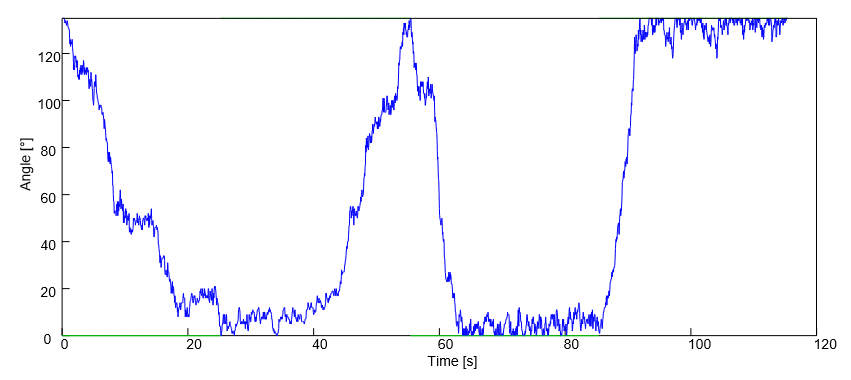
\includegraphics[width=0.7\linewidth]{figures/ModelSebastian/ExemplarLearning}
	\caption[Exemplar Learning Phase]{\textbf{Exemplar Learning Phase:} Starting from angle 135\degree, the angles 0\degree and 135\degree have to be reached. This example needs 50 seconds to achieve this. During this 50 seconds learning is enabled. Afterwards it is checked whether the model is able to reach the minimal an maximal angle without learning. Both angles are applied as target angles for 30 seconds. Not that time is referred to as simulation time not as actual time. \cite[p. 47]{sebastianMasterThesis}}
	\label{fig:exemplarlearning}
\end{figure}
%TODO show movement and D spikning together if possible. Sebastian fragen ""

\begin{figure}[tb]
	\centering
	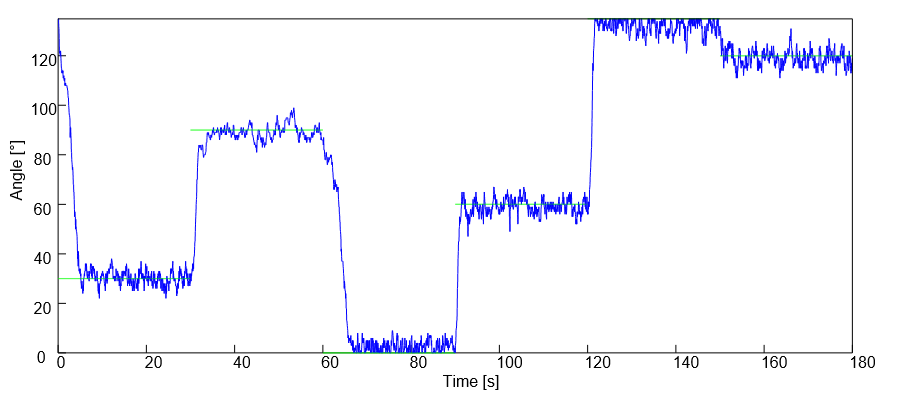
\includegraphics[width=0.7\linewidth]{figures/ModelSebastian/LowestOverallRMSD}
	\caption[Spüler's Lowest Overall RMSD]{\textbf{Spüler's simulation with lowest Overall RMSD:} After learning the model gets tested in a simulation where several angles have to be reached. Starting with 135\degree consecutively 30\degree,90\degree,0\degree,60\degree,135\degree and 120\degree have to be reached. Each target angle is presented for 30 seconds. This model is the best performing model found by Spüler et al. with an RMSD of 3.3\degree. \cite[p. 52]{sebastianMasterThesis}}
	\label{fig:lowestoverallrmsd}
\end{figure}
%TODO sebastian frage weil rmsd zu niedrig 


\begin{figure}[tb]
	\centering
	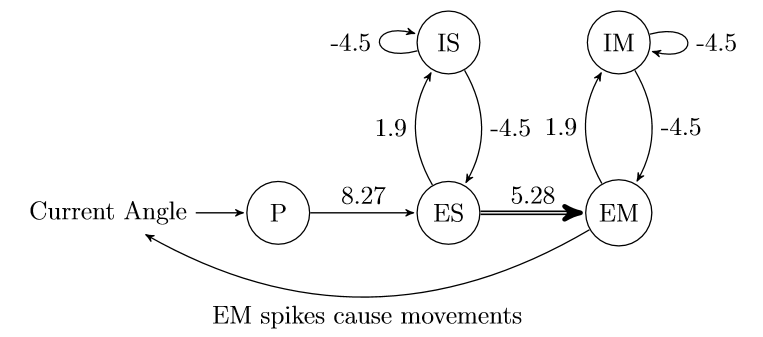
\includegraphics[width=0.7\linewidth]{figures/ModelSebastian/OngoingModelStructure}
	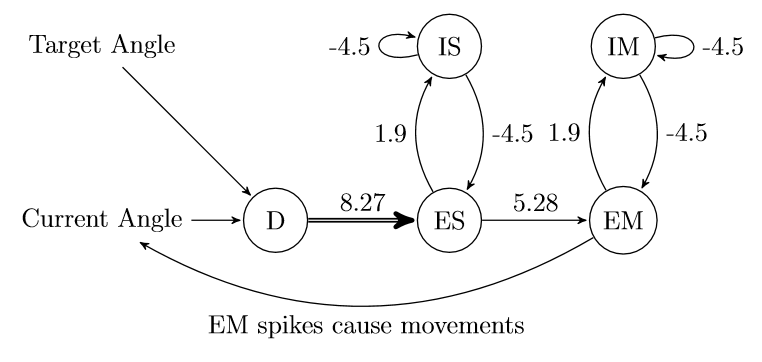
\includegraphics[width=0.7\linewidth]{figures/ModelSebastian/StaticModelStructur}
	\caption[Spüler et al. actor model structures]{\textbf{Spüler et al. actor model structures:} The upper figure shows the structure of the Ongoing Learning Model. The lower figure the structure of the Static Learning Models. Each circle represents a cell type. Each arrow represents a connection probability greater 0. The double lined arrow represents inter cell connections where learning is applied. \cite[p. 25,41]{sebastianMasterThesis}}
	\label{fig:modelstructur}
\end{figure}


\begin{figure}[tb]
	\centering
	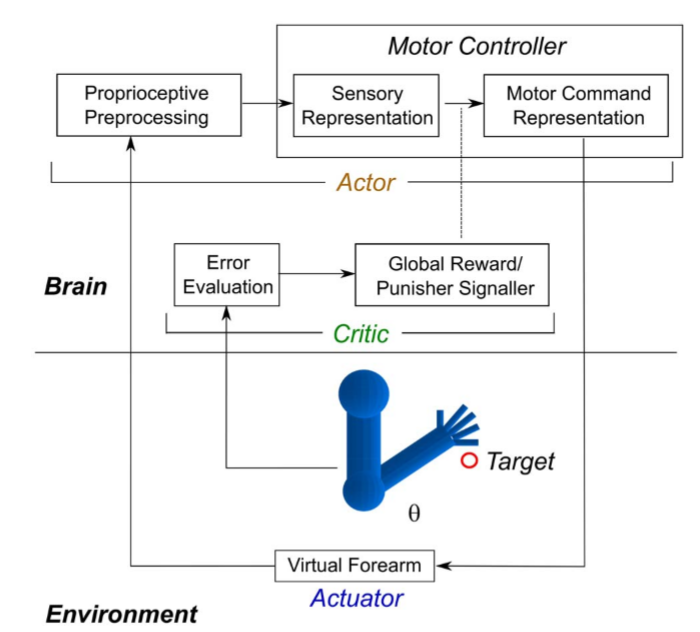
\includegraphics[width=0.7\linewidth]{figures/ModelSebastian/ReinforcementCircle}
	\caption[Spüler et al. whole model design]{\textbf{Spüler et al. whole model design:} This figure gives an whole overview over Spüler et al.'s model components and its reinforcement learning circle. The critic and actor ar parts of the brain (or more general the learning system). The forearm is part of the environment. A detailed view of the actor's structure can be found in \ref{fig:staticmodelstructur}. \cite[p. 3]{chadderdonNeuronalModel}.
.	\label{fig:reinforcementcircle}
\end{figure}

\begin{figure}
	\centering
	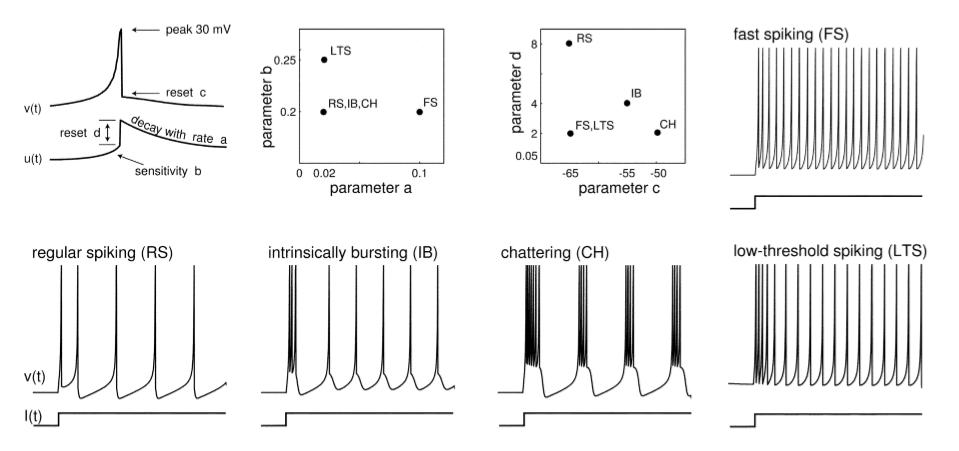
\includegraphics[width=0.7\linewidth]{figures/ModelSebastian/SpikingPatterns}
	\caption[Izhikevich simple \cite{izhikevichSimpleModel} model spiking patterns]{\textbf{Izhikevich simple model \cite{izhikevichSimpleModel} spiking patterns}. Different resulting spiking patterns by variation of $a,b,c,d=V_r$ patterns. The here depicted patterns are correspond to known biological neuron types. RS, IB and CH are cortical excitatory neurons. FS and LTS are cortical inhibitory neurons. Time resolution is 0.1ms. Each pattern is initialized by a dc-current (I) step from 0 to 10. \cite{izhikevichSimpleModel}}  %unit unknown ma or A ?
	\label{fig:spikingpatterns}
\end{figure}

\begin{figure}
	\centering
	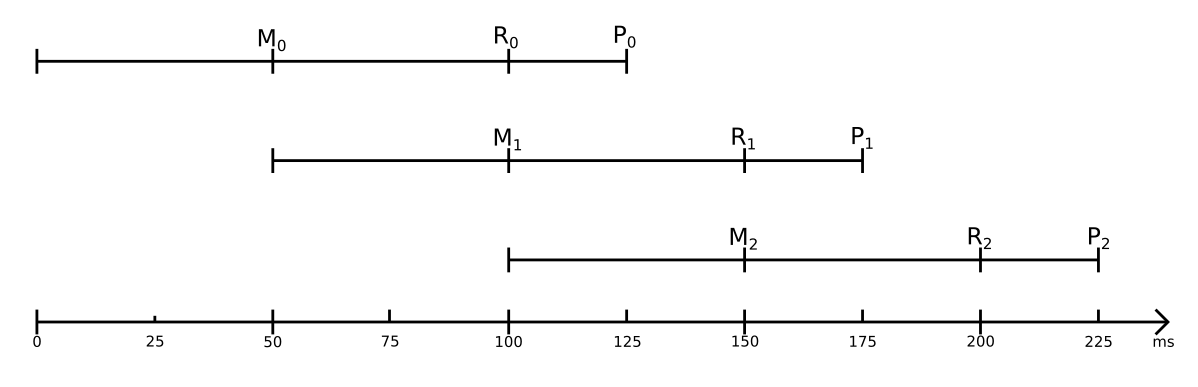
\includegraphics[width=0.7\linewidth]{figures/ModelSebastian/timing}
	\caption[Motor Control cycles]{\textbf{3 exemplar consecutive motor control cycles. Until M a new motor signal gets encoded by EM cells. Than until R there is a 50ms time gap. At R the motor arm is moved and the critic responses. After 25 more milliseconds the new position is encoded by the P cells. Note that P cells get activated during the encoding of the next motor command. The time gaps are biological founded by Spüler et al as peripheral and subcortical delay times.}}
	\label{fig:timing}
\end{figure}

\begin{figure}[tb]
	\centering
	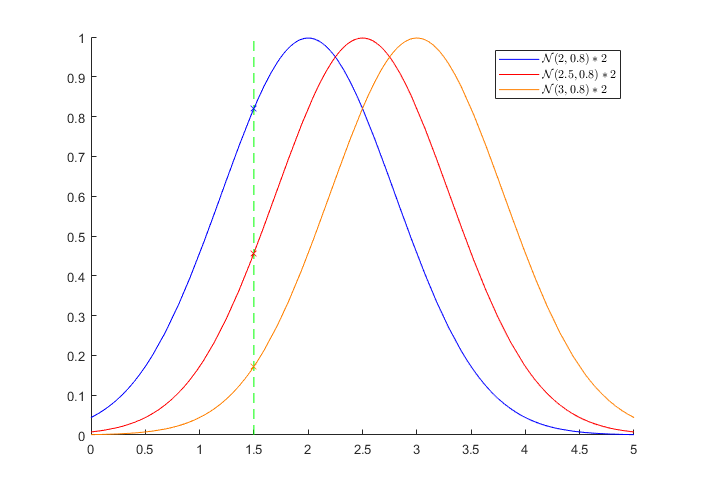
\includegraphics[width=0.7\linewidth]{figures/ModelSebastian/popCode}
	\caption[Population Coding]\textbf{Exemplar Population coding by D cells}. Here the normal distributions of activation probabilities for neurons at 2 (blue), 2.5 (red) and 3(orange) are shown. The dashed green line marks the position of an angle to encode. Note that every cell will fire with a different probability. ($P(blue)=0.8204$, $P(red)=0.4566$, $P(orange)=0.1720$)   }
	\label{fig:popCode}
\end{figure}



TODO population coding of P cells.
TODO picture structure done
TODO Own plot time.

TODO Appendix picture weight formula todo. 
TODO fireing patters. todo
